\documentclass[12pt]{article}
\usepackage[margin=3cm]{geometry}
\usepackage{graphicx}
\usepackage{float}
\usepackage{url}
\usepackage{listings}
\usepackage{color}

\definecolor{mygreen}{rgb}{0,0.6,0}
\definecolor{mygray}{rgb}{0.5,0.5,0.5}
\definecolor{mymauve}{rgb}{0.58,0,0.82}
\lstset{ %
	xleftmargin=15em,
	backgroundcolor=\color{white},   % choose the background color; you must add \usepackage{color} or \usepackage{xcolor}
	basicstyle=\small,%\footnotesize,        % the size of the fonts that are used for the code
	breakatwhitespace=false,         % sets if automatic breaks should only happen at whitespace
	breaklines=false,                 % sets automatic line breaking
	captionpos=b,                    % sets the caption-position to bottom
	commentstyle=\color{mygreen},    % comment style
	deletekeywords={...},            % if you want to delete keywords from the given language
	escapeinside={\%*}{*)},          % if you want to add LaTeX within your code
	extendedchars=true,              % lets you use non-ASCII characters; for 8-bits encodings only, does not work with UTF-8
	%	frame=single,                    % adds a frame around the code
	keepspaces=true,                 % keeps spaces in text, useful for keeping indentation of code (possibly needs columns=flexible)
	keywordstyle=\color{blue},       % keyword style
	language=C, % the language of the code
	morekeywords={*,...},            % if you want to add more keywords to the set
	numbers=left,                    % where to put the line-numbers; possible values are (none, left, right)
	numbersep=5pt,                   % how far the line-numbers are from the code
	numberstyle=\small\color{mygray}, % the style that is used for the line-numbers
	rulecolor=\color{black},         % if not set, the frame-color may be changed on line-breaks within not-black text (e.g. comments (green here))
	showspaces=false,                % show spaces everywhere adding particular underscores; it overrides 'showstringspaces'
	showstringspaces=false,          % underline spaces within strings only
	showtabs=false,                  % show tabs within strings adding particular underscores
	stepnumber=1,                    % step between two line-numbers. If it's 1, each line will be numbered
	stringstyle=\color{mymauve},     % string literal style
	tabsize=2                  % sets default tabsize to 2 spac                  % show the filename of files included with \lstinputlisting; also try caption instead of title
}

\begin{document}

\begin{titlepage}
	\begin{center}
		
		
		% Upper part of the page. The '~' is needed because \\
		% only works if a paragraph has started.
		\vfill
		
		\textsc{\LARGE Lab 6: Carry-Ripple Addition I}\\[1.5cm]
		
		\Large Adam Sumner\\[0.5cm]
		
		\Large Illinois Institute of Technology\\[0.5cm]
		
		\Large ECE 429-01\\[0.5cm]	
		
		\noindent
		\vfill
		\large \textbf{Lab Date:} October 19\textsuperscript{th}, 2015\hfill
		\large \textbf{Due Date:} October 28\textsuperscript{th}, 2015
		% Bottom of the page
	
		
	\end{center}
\end{titlepage}

\section{Introduction}
The purpose of this lab is to design the schematic of a full binary adder. A test circuit will  be used to verify the results, along with equivalence checking against a full adder implemented in the Verilog hardware description language. 
\section{Theory/Pre-Lab}
\subsection{Theory}
When calculating the addition of two binary numbers, the addition is performed bit-by-bit. For example, in the addition of two numbers A+B, let A and B be bit strings of the same length, let S be the sum of the operation, and let C be the carry bit generated from the ith bit in each individual bit addition. The addition can be computed as follows:
$$C[0]=0$$
$$S[i]=A[i] \ XOR \ B[i]  \ XOR \ C[i]$$
$$C[i+1]=A[i]B[i] + A[i]C[i]+B[i]C[i]$$

\noindent where $i \geq 0$. While several architectures have been proposed to implement this full adder functionality, the primary design that reduces the number of transistors required and also increases the speed of the addition operation is the mirror adder shown in Figure \ref{fig:mirror-pre}. The mirror adder exploits the following two sets of equations of S and C to construct the pull-up and pull-down networks that are symmetrical to each other:

$$\textrm{pull-up network}:c_{output}=(a+b)(ab+c_{input}),\ S=(a+b+c_{input})(a\cdot b \cdot c_{input}+c_{output})$$
$$\textrm{pull-down network}: c_{output}=a \cdot b+(a+b)c_{input},\ S=a\cdot b\cdot c_{input}+(a+b+c_{input})c_{output}$$
\\
\noindent To verify the functionality of any full-adder design, the following Verilog code can be used:
\begin{figure}[H]
\begin{lstlisting}
module 
	adder(ab,ci,s,co);
	input a,b,ci;
	output s,co;
	assign s=a^b^ci;
	assign co=(a&b)|(b&ci)|(ci&a);
endmodule
\end{lstlisting}
\caption{Verilog Code for Full-Adder Verification}
\label{fig:verilog}
\end{figure}
\begin{figure}[H]
\centering
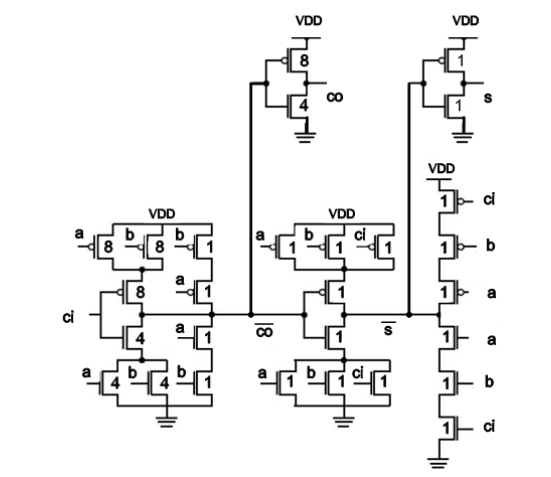
\includegraphics[width=0.7\linewidth]{mirror-pre}
\caption{Mirror Adder Design}
\label{fig:mirror-pre}
\end{figure}
\subsection{Pre-Lab}
The pre-lab involved studying the schematic shown in Figure \ref{fig:mirror-pre}. This design was successfully explored.
\section{Implementation}
\subsection{Schematics}
\begin{figure}[H]
\centering
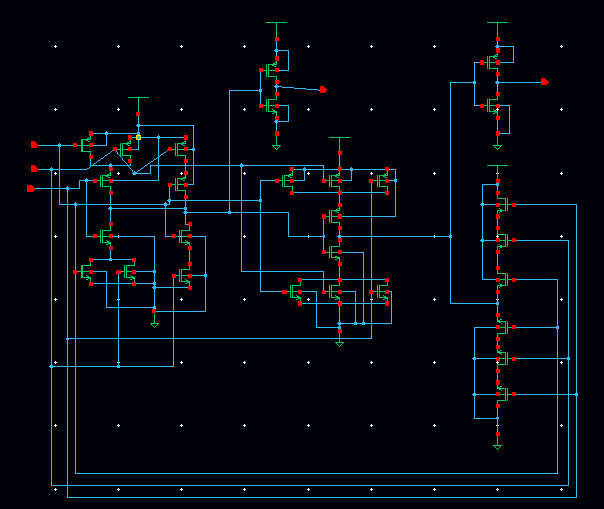
\includegraphics[width=1\linewidth]{mirror-schematic}
\caption{Mirror Schematic Implementation}
\label{fig:mirror-schematic}
\end{figure}

\begin{figure}[H]
\centering
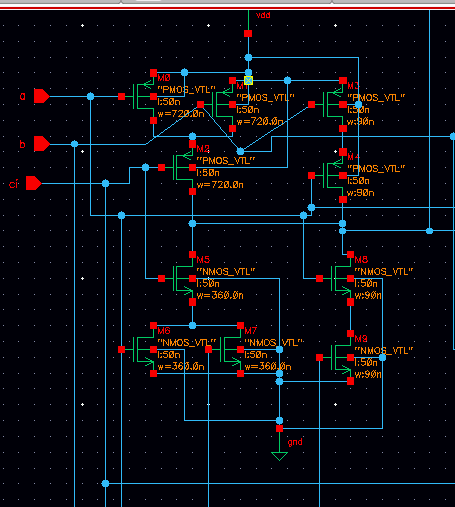
\includegraphics[width=\linewidth]{schematic-closeup-1}
\caption{Schematic Closeup 1}
\label{fig:schematic-closeup-1}
\end{figure}


\begin{figure}[H]
\centering
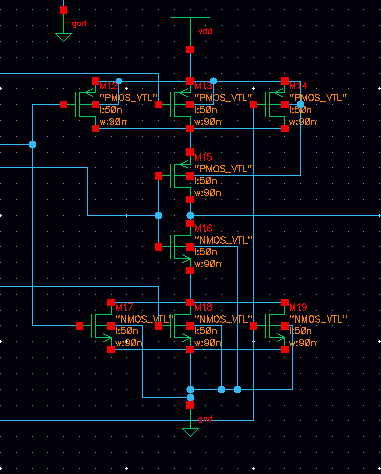
\includegraphics[width=\linewidth]{schematic-closeup-2}
\caption{Schematic Closeup 2}
\label{fig:schematic-closeup-2}
\end{figure}

\begin{figure}[H]
\centering
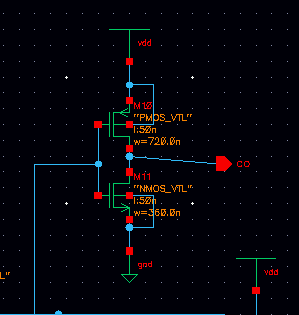
\includegraphics[width=0.5\linewidth]{schematic-closeup-3}
\caption{Schematic Closeup 3}
\label{fig:schematic-closeup-3}
\end{figure}

\begin{figure}[H]
\centering
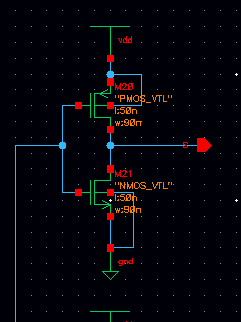
\includegraphics[width=0.5\linewidth]{schematic-closeup-4}
\caption{Schematic Closeup 4}
\label{fig:schematic-closeup-4}
\end{figure}
\begin{figure}[H]
\centering
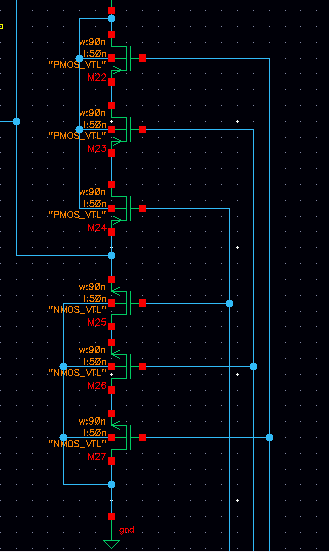
\includegraphics[width=0.5\linewidth]{schematic-closeup-5}
\caption{Schematic Closeup 5}
\label{fig:schematic-closeup-5}
\end{figure}

\begin{figure}[H]
\centering
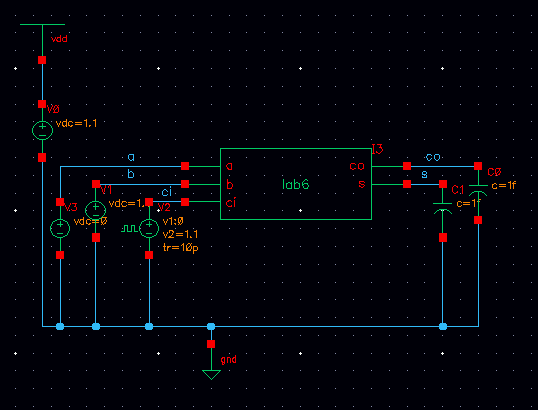
\includegraphics[width=1\linewidth]{test-circuit}
\caption{Test Circuit for Mirror Adder}
\label{fig:test-circuit}
\end{figure}


\subsection{Procedure}
The schematic of the mirror adder in Figure \ref{fig:mirror-pre} was implemented in virtuoso. The final design is shown in Figure \ref{fig:mirror-schematic}. After this, a symbol was generated for the full adder and then a test circuit was made. This is shown in figure \ref{fig:test-circuit}. Once complete, the netlist was generated and stored in a file called \texttt{lab6.sp}. This file was used with the Verilog file shown in Figure \ref{fig:verilog} to validate the functionality of the implemented schematic. After this, the delay between $c_i$ and $c_o$ was calculated.
\subsection{Results}

\begin{figure}[H]
\centering
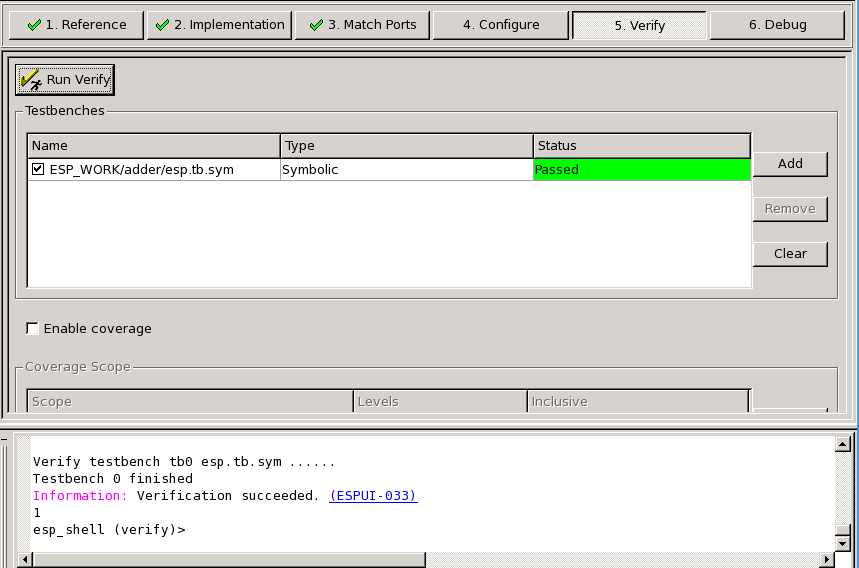
\includegraphics[width=1\linewidth]{verification}
\caption{ESP Verification of Implemented Mirror Adder and Verilog Adder}
\label{fig:verification}
\end{figure}

\begin{figure}[H]
\centering
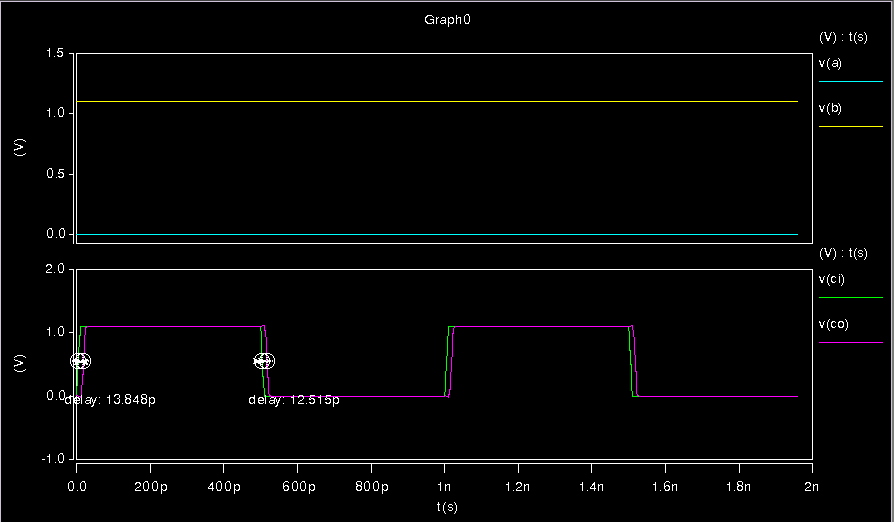
\includegraphics[width=\linewidth]{010-011}
\caption{Delay for $010 \to 011\ 011 \to 010$}
\label{fig:010-011}
\end{figure}

\begin{figure}[H]
\centering
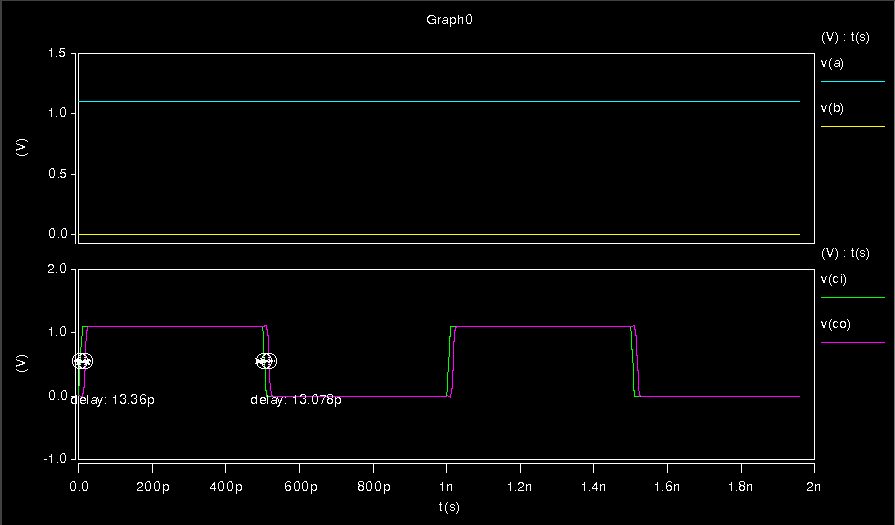
\includegraphics[width=1\linewidth]{100-101}
\caption{Delay for $100 \to 101 \ 101 \to 100$}
\label{fig:100-101}
\end{figure}

Figures \ref{fig:010-011} and \ref{fig:100-101} show delays between $c_i$ and $c_o$ of 13.848p s and 13.36 p s rising and 12.515p s and 13.078p s falling respectively.

\subsection{Discussion}
After spending hours implementing the mirror adder schematic, it is clear from Figure \ref{fig:verification} that it indeed functions as it should. Once the functionality was confirmed, the test circuit results of the delay between $c_i$ and $c_o$ were measured and the results are shown in Figures \ref{fig:010-011} and \ref{fig:100-101}. Considering the size and complexity of this circuit, the delay is at an acceptable minimum. This is due to the correct sizing of each transistor in the circuit. When minimizing delay, it is critical to size transistors so that they follow the ratio of the standard inverter implementation. This ratio is 2:1 where PMOS has a width double that of the NMOS transistor. According to the sizes in Figure \ref{fig:mirror-pre}, values for 4 and 8 were 360nm 720nm respectively. This is because the base size used in our design was 90nm. Furthermore $c_i$ was used as the inner inputs because this results in the biggest reduction in delay for the signal.

	
%\subsection{Bonus Work}
\section{Conclusions}
Overall the lab was a success. A full adder schematic was successfully implemented and verified using a Verilog adder file. Furthermore the delay between the carry in and carry out bits were successfully calculated and were accurate. This schematic can now be used in the future to design the physical layout.

\end{document}
